\chapter{Thực nghiệm, kết quả và thảo luận}
\label{ch:thuc-nghiem}
% Nguồn: runs/ và các bảng sinh bởi report/scripts/phan-tich-tong-hop.py.
% Mỗi bảng ghi rõ cỡ mẫu; không cộng các nguồn dùng chung khai cuộc.

Chương này trình bày kết quả thực nghiệm theo bốn lớp: (i) giải vòng tròn tám tác tử và các
đối chứng trực tiếp; (ii) các thí nghiệm phân tích thành phần; (iii) đường cong huấn luyện và
chất lượng mô hình học được; (iv) phân tích ván, phân loại lỗi và chi phí. Mỗi mục nêu thiết
lập, số liệu, cách đọc và giới hạn của phép đo. Các kết luận được tổng hợp ở
Mục~\ref{sec:tn-tra-loi-rq} và Chương~\ref{ch:ket-luan}.

\section{Môi trường và nguồn số liệu}
\label{sec:tn-moi-truong}
\subsection{Phần cứng, phần mềm và cách chạy}
Các phép đo chính chạy trên một máy laptop: Intel Core i7-11800H (8 nhân, 16 luồng), 16 GB RAM,
GPU NVIDIA RTX A2000 Laptop 4 GB, Python 3.13.16, PyTorch 2.14.1 với CUDA 13.0. Hệ điều hành
là Linux Fedora. Các run cũ hơn có thể chạy trên cấu hình khác; báo cáo chỉ so sánh thời gian
giữa các tác tử trong cùng một run hoặc cùng một cấu hình, không so thời gian tuyệt đối giữa
các run khác máy.

Mọi run ghi \texttt{meta.json} gồm commit Git, cờ dirty, phiên bản Python và thư viện, CPU,
RAM, GPU, seed và hash cấu hình. Khi working tree dirty, log ghi rõ; các run này được đánh dấu
là bằng chứng phụ nếu có run sạch tương đương. Bảng~\ref{tab:tn-nguon} liệt kê các nguồn số
liệu chính và quy mô.

\begin{table}[H]
  \centering\small
  \caption{Các nguồn số liệu chính. Các nguồn có thể dùng chung khai cuộc; không cộng chúng để
  suy ra cỡ mẫu độc lập.}
  \label{tab:tn-nguon}
  \begin{tabularx}{\textwidth}{@{}lXl@{}}
    \toprule
    \textbf{Nguồn} & \textbf{Đơn vị so sánh} & \textbf{Quy mô} \\
    \midrule
    RR8 (mới) & Tám tác tử, 50 khai cuộc đổi màu & 2\,800 ván \\
    E3 (mới) & Mỗi cấp tự đấu, 50 khai cuộc đổi màu & 800 ván \\
    A7b (mới) & Hai bảng trọng số Alpha-Beta, độ sâu 4 & 100 ván \\
    A1 & Cắt tỉa bật/tắt trên 50 thế cờ & 50 thế $\times$ 3 lần \\
    A2 & Sắp xếp nước và TT trên 10 thế, ngân sách 1 s & 10 thế $\times$ 3 lần \\
    A7 & Trọng số mặc định/bỏ phòng thủ trên 10 thế & 10 thế $\times$ 3 lần \\
    A3 & MCTS 100/400/1600/6400 mô phỏng gặp L2, L3 & 1\,600 ván \\
    A4 & MCTS rollout ngẫu nhiên/nhẹ gặp L2, L3 & 800 ván \\
    A5 & Policy-only, PUCT và các mốc mô phỏng & 2\,200 ván \\
    Arena cũ & Sáu cấu hình L1--L5, mỗi tác tử 500 ván & 1\,500 ván \\
    L6 & 49\,920 episode tự đấu, 10 mốc đánh giá & 10 mốc \\
    L8 & 50 vòng, 10\,000 ván tự đấu, 6 lần duyệt & 50 vòng \\
    L8--L7, L8--L3 & Cùng ngân sách, đổi màu & 20 + 40 ván \\
    \bottomrule
  \end{tabularx}
\end{table}

\subsection{Ba mức bằng chứng}
Báo cáo phân biệt ba mức. \emph{Bằng chứng chính} là run có \texttt{summary.json} trạng thái
\texttt{ok}, cấu hình đầy đủ, seed cố định và log ván đầy đủ. \emph{Bằng chứng phụ} là run bị
ngắt, dirty hoặc thiếu trường, chỉ dùng minh hoạ. \emph{Quan sát} là phân tích trên log cũ,
có thể chịu ảnh hưởng của phiên bản code khác. Khi một kết luận chỉ dựa trên bằng chứng phụ
hoặc quan sát, câu văn ghi rõ. Cách phân loại này quan trọng vì dự án phát triển song song với
việc chạy thực nghiệm: một số log được tạo trước khi sửa lỗi quy ước value, hoặc trước khi
chuyển sang backend Cython.

\subsection{Cách đọc bảng}
Trong các bảng đấu, W/D/L là thắng/hoà/thua từ góc nhìn tác tử ở hàng. Điểm là
$(W+0.5D)/n$. Khoảng Wilson 95\% dùng cho từng tỷ lệ; khoảng bootstrap theo cặp khai cuộc dùng
khi cần so sánh tổng thể. Các cột thời gian là mili giây mỗi nước, đo bên ngoài lời gọi tác tử,
gồm cả chi phí sao chép trạng thái. Cột mô phỏng/nút là trung bình trên các nước của tác tử đó,
không gồm nước khai cuộc.

\section{Giải vòng tròn tám tác tử}
\label{sec:tn-rr8}
\subsection{Thiết lập}
RR8 cho tám tác tử gặp nhau theo thể thức vòng tròn, 50 khai cuộc, mỗi khai cuộc hai ván đổi
màu. Mỗi cặp có 100 ván; toàn giải 2\,800 ván. Ngân sách cố định theo loại thuật toán:
Alpha-Beta độ sâu 4, MCTS 400 mô phỏng, PUCT 200 mô phỏng, policy-only argmax. Đây là ngân sách
đủ nhỏ để chạy trên một máy cá nhân, nhưng đủ lớn để các khác biệt về tri thức chiến thuật lộ
ra. Chi tiết cấu hình ở Mục~\ref{sec:pp-rr8}.

\subsection{Xếp hạng, ma trận và khoảng tin cậy}
\begin{table}[H]
  \centering\small
  \caption{Xếp hạng RR8 (trên) và ma trận điểm phần trăm của tác tử hàng trước tác tử cột
  (dưới). Mỗi ô ma trận dựa trên 100 ván; dấu ``—'' là tự đấu.}
  \label{tab:tn-rr8}
  \begin{center}\small
\begin{tabular}{@{}lrrrr@{}}
\toprule
Tác tử & Ván & W/D/L & Điểm & Wilson 95\% \\
\midrule
L8-AlphaZero & 700 & 616/25/59 & 89,8\% & [87,3\%; 91,8\%] \\
L7-PUCT & 700 & 566/16/118 & 82,0\% & [79,0\%; 84,7\%] \\
L6-PolicyRL & 700 & 421/24/255 & 61,9\% & [58,2\%; 65,4\%] \\
L3-AlphaBeta & 700 & 392/32/276 & 58,3\% & [54,6\%; 61,9\%] \\
L5-PolicySL & 700 & 348/7/345 & 50,2\% & [46,5\%; 53,9\%] \\
L2-Rule & 700 & 300/10/390 & 43,6\% & [39,9\%; 47,3\%] \\
L4-MCTS & 700 & 100/0/600 & 14,3\% & [11,9\%; 17,1\%] \\
L1-Random & 700 & 0/0/700 & 0,0\% & [0,0\%; 0,5\%] \\
\bottomrule
\end{tabular}
\end{center}
\begin{center}\scriptsize\setlength{\tabcolsep}{3pt}
\begin{tabular}{@{}lcccccccc@{}}
\toprule
 & L1-Random & L2-Rule & L3-AlphaBeta & L4-MCTS & L5-PolicySL & L6-PolicyRL & L7-PUCT & L8-AlphaZero \\
\midrule
L1-Random & — & 0 & 0 & 0 & 0 & 0 & 0 & 0 \\
L2-Rule & 100 & — & 37 & 100 & 32 & 20 & 12 & 4 \\
L3-AlphaBeta & 100 & 63 & — & 100 & 64 & 46 & 22 & 13 \\
L4-MCTS & 100 & 0 & 0 & — & 0 & 0 & 0 & 0 \\
L5-PolicySL & 100 & 68 & 36 & 100 & — & 37 & 5 & 5 \\
L6-PolicyRL & 100 & 80 & 54 & 100 & 63 & — & 21 & 16 \\
L7-PUCT & 100 & 88 & 78 & 100 & 95 & 79 & — & 34 \\
L8-AlphaZero & 100 & 96 & 87 & 100 & 95 & 84 & 66 & — \\
\bottomrule
\end{tabular}
\end{center}
\end{table}

Bảng xếp hạng tách thành bốn nhóm. Nhóm dẫn đầu gồm L8 AlphaZero (89,8\%) và L7 PUCT (82,0\%);
khoảng Wilson của hai tác tử này không chồng lấn với phần còn lại. Nhóm giữa gồm L6 PolicyRL
(61,9\%), L3 Alpha-Beta (58,3\%), L5 PolicySL (50,2\%) và L2 Rule (43,6\%); khoảng tin cậy của
L6 và L3 chồng lấn nhẹ, của L3 và L5 gần chạm nhau, còn L2 thấp hơn (khoảng tin cậy chỉ chạm
nhẹ L5). Nhóm cuối gồm L4 MCTS
(14,3\%) và L1 Random (0,0\%).

Ba kết quả đáng chú ý. Thứ nhất, PUCT với mạng học được vượt Alpha-Beta viết tay rất xa: L7
82,0\% so với L3 58,3\%, chênh 23,7 điểm phần trăm, khoảng tin cậy tách rời. Đây là bằng chứng
mạnh nhất cho RQ2 trong giải mới. Thứ hai, RL vượt SL: L6 61,9\% so với L5 50,2\%, và L6 nhỉnh
hơn L3 dù chỉ 3,6 điểm phần trăm (khoảng tin cậy chồng lấn, nên chưa thể khẳng định L6 mạnh
hơn L3 một cách chắc chắn). Thứ ba, MCTS thuần thua cả tác tử luật: L4 14,3\% so với L2 43,6\%.
Đây không phải vì MCTS ``kém'' nói chung, mà vì ở ngân sách 400 mô phỏng và rollout ngẫu nhiên,
nó không thấy được các chuỗi ép ngắn; nguyên nhân được phân tích ở Mục~\ref{sec:tn-mcts} và
Mục~\ref{sec:tn-loi}.

Ma trận đối đầu cho thấy vài bất thường cục bộ. L8 thắng L7 66\%, nhưng L7 thắng L3 78\% và
thắng L6 79\%; L6 thắng L3 54\% nhưng thua L3 ở một số khai cuộc. L5 thắng L2 68\% nhưng chỉ
thắng L3 36\%. L4 thắng L1 100\% nhưng thua tất cả các tác tử còn lại. Các chuỗi này nhắc rằng
điểm tổng không đủ để mô tả quan hệ đối đầu; cần đọc cả ma trận và khoảng tin cậy.

\subsection{Điểm theo màu}
\begin{figure}[H]
  \centering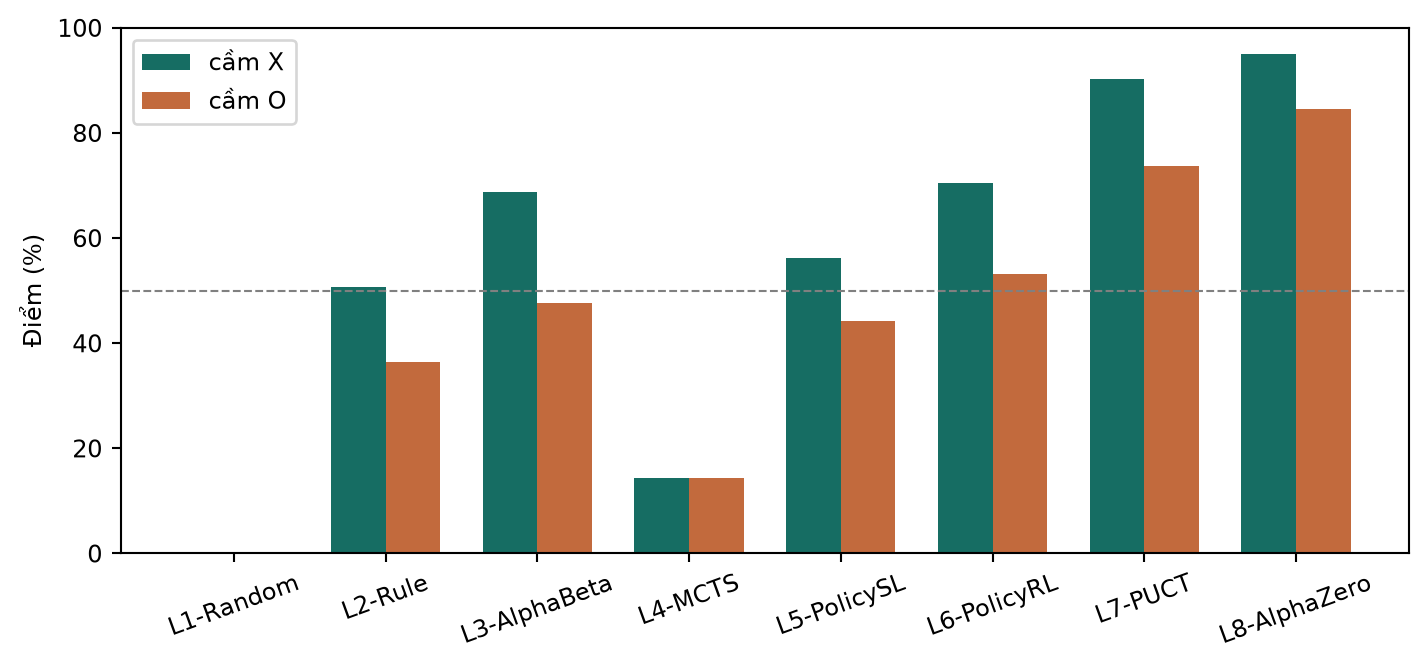
\includegraphics[width=.9\textwidth]{ban-mo-rong/hinh/rr8_color.png}
  \caption{Điểm của từng tác tử khi cầm X và khi cầm O trong RR8. Điểm tính cả hoà nửa điểm.}
  \label{fig:tn-rr8-color}
\end{figure}
Mỗi tác tử được tách theo màu X (đi trước) và O (đi sau). Mọi tác tử đều đạt điểm cao hơn khi
cầm X, nhưng mức chênh khác nhau: L8 95,0\% so với 84,6\% (chênh 10,4 điểm phần trăm), L7 90,3\%
so với 73,7\% (16,6), L3 68,9\% so với 47,7\% (21,2), L6 70,6\% so với 53,1\% (17,5), L5 56,1\%
so với 44,3\% (11,8), L2 50,7\% so với 36,4\% (14,3). L4 và L1 bằng nhau ở hai màu vì chúng
thua gần như mọi đối thủ bất kể màu.

Điều này cho thấy lợi thế đi trước không biến mất khi tác tử mạnh lên. L8 vẫn thắng 95,0\% khi
cầm X và 84,6\% khi cầm O; khoảng cách 10,4 điểm là nhỏ hơn L3 (21,2) nhưng không bằng 0. Cách
hiểu hợp lý là tác tử mạnh hơn có thể \emph{giảm} khoảng cách bằng cách phòng thủ tốt hơn khi
cầm O, chứ không phải xoá bỏ lợi thế. Đây là lý do mọi giải trong báo cáo đều đổi màu.

\subsection{Độ dài ván}
\begin{figure}[H]
  \centering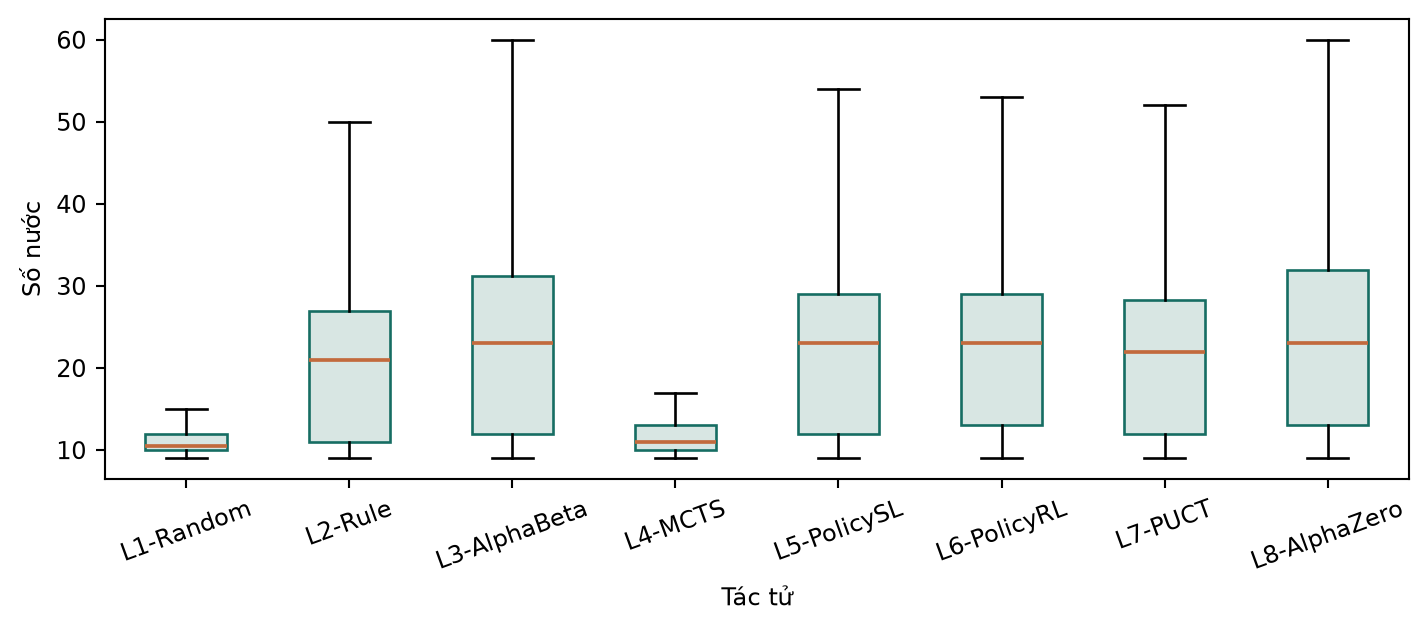
\includegraphics[width=.9\textwidth]{ban-mo-rong/hinh/rr8_lengths.png}
  \caption{Phân bố độ dài ván của từng tác tử trong RR8 (hộp 25--75\%, trung vị màu cam).}
  \label{fig:tn-rr8-length}
\end{figure}
Phân bố độ dài ván phản ánh phong cách. L1 và L4 có trung vị ngắn nhất (10 và 11 nước) vì
ván kết thúc nhanh khi một bên vô tình hoặc bỏ sót tạo ra năm quân. L2, L3, L5, L6, L7 và L8
có trung vị 21--23 nước; đuôi phân bố khác nhau: L3 có p95 73 nước, L8 66, L6 61, L7 54, L5 48,
L2 44. Đuôi dài xuất hiện khi cả hai bên phòng thủ tốt và ván kéo đến gần đầy bàn. Đuôi này
quan trọng hơn trung vị khi đánh giá chi phí, vì một ván dài làm tăng thời gian chạy nhưng
không nhất thiết làm tăng chất lượng.

\subsection{Khai cuộc và phương sai}
\begin{table}[H]
  \centering\small
  \caption{Điểm theo khai cuộc: trung bình, độ lệch chuẩn và ba khai cuộc tốt/xấu nhất của từng
  tác tử trong RR8.}
  \label{tab:tn-khai-cuoc}
  \begin{center}\footnotesize
\setlength{\tabcolsep}{4pt}
\begin{tabularx}{\textwidth}{@{}lrrr>{\raggedright\arraybackslash}X>{\raggedright\arraybackslash}X@{}}
\toprule
\textbf{Tác tử} & \textbf{Khai cuộc} & \textbf{Điểm TB} & \textbf{Độ lệch} & \textbf{3 tốt nhất} & \textbf{3 xấu nhất} \\
\midrule
L1-Random & 50 & 0,000 & 0,000 & 0:0\%, 1:0\%, 2:0\% & 0:0\%, 1:0\%, 2:0\% \\
L2-Rule & 50 & 0,436 & 0,086 & 7:64\%, 25:64\%, 40:64\% & 29:29\%, 38:29\%, 35:32\% \\
L3-AlphaBeta & 50 & 0,583 & 0,087 & 41:79\%, 31:75\%, 16:71\% & 17:36\%, 36:39\%, 9:43\% \\
L4-MCTS & 50 & 0,143 & 0,000 & 0:14\%, 1:14\%, 2:14\% & 0:14\%, 1:14\%, 2:14\% \\
L5-PolicySL & 50 & 0,502 & 0,083 & 9:71\%, 26:71\%, 43:68\% & 7:36\%, 16:36\%, 25:36\% \\
L6-PolicyRL & 50 & 0,619 & 0,097 & 6:86\%, 8:82\%, 45:82\% & 12:43\%, 19:43\%, 31:46\% \\
L7-PUCT & 50 & 0,820 & 0,079 & 46:100\%, 38:96\%, 11:93\% & 14:68\%, 7:71\%, 15:71\% \\
L8-AlphaZero & 50 & 0,898 & 0,078 & 2:100\%, 4:100\%, 15:100\% & 40:71\%, 6:75\%, 9:79\% \\
\bottomrule
\end{tabularx}
\end{center}
\end{table}
Bảng khai cuộc cho thấy điểm của cùng một tác tử vẫn dao động giữa các khai cuộc, nhưng ít hơn
so với điểm từng cặp: độ lệch chuẩn 0,078--0,097 vì mỗi ô đã trung bình trên 7 đối thủ (14
ván). Vẫn có những khai cuộc tác tử thắng gần như chắc chắn và những khai cuộc thua gần như
chắc chắn. Ví dụ, L8 đạt 100\% ở các khai cuộc 2, 4, 15 nhưng chỉ 71--79\% ở các khai cuộc 40,
6, 9; L3 đạt 79\% ở khai cuộc 41 nhưng 36\% ở khai cuộc 17. Với L4, mọi khai cuộc đều 14,3\%
vì nó thua tất cả các đối thủ trừ L1.

Hai hệ quả. Thứ nhất, so sánh hai tác tử trên một khai cuộc duy nhất gần như vô nghĩa. Thứ hai,
khoảng tin cậy theo cặp khai cuộc rộng hơn khoảng Wilson từng ván, vì nó phản ánh đúng sự phụ
thuộc giữa hai ván của cùng khai cuộc. Đây là lý do báo cáo dùng 50 khai cuộc và bootstrap theo
cặp, không chỉ Wilson trên tổng số ván.

\subsection{Đọc kết quả RR8}
Có năm quan sát chính. Thứ nhất, PUCT có mạng học vượt Alpha-Beta viết tay rất xa: L7 82,0\% và
L8 89,8\% so với L3 58,3\%. Đây là kết quả mạnh nhất của giải mới và là bằng chứng trực tiếp cho
RQ2. Thứ hai, RL vượt SL: L6 61,9\% so với L5 50,2\%, chênh 11,7 điểm phần trăm; L6 thậm chí
nhỉnh hơn L3 3,6 điểm, dù khoảng tin cậy chồng lấn nên chưa thể khẳng định. Thứ ba, SL một mình
không đủ: L5 chỉ 50,2\%, thấp hơn L3 8,1 điểm; policy học bắt chước cần tìm kiếm để bù các lỗi
chiến thuật. Thứ tư, MCTS thuần yếu hơn cả tác tử luật: L4 14,3\% so với L2 43,6\%, vì rollout
ngẫu nhiên ở 400 mô phỏng không đủ thấy chuỗi ép 4 ply. Thứ năm, chi phí không tỷ lệ với sức
mạnh: L7/L8 mất khoảng 37 ms/nước trung vị, L4 mất 64 ms, L3 chỉ 5,2 ms, L5/L6 1,3 ms. L4 là
ví dụ rõ nhất của ``tốn thời gian nhưng không hiệu quả'' trong cấu hình này.

Phân tích chiến thuật củng cố các quan sát trên. L2 và L3 không bỏ cơ hội thắng/chặn nào trong
hàng nghìn nước. L4 bỏ 227/327 cơ hội thắng ngay và 50/57 cơ hội chặn. L5 bỏ 54/402 cơ hội
thắng nhưng 0/941 cơ hội chặn; L6 bỏ 22/443 và 17/1131. L7 bỏ 19/585 và 24/973; L8 bỏ 5/621 và
6/1277. Hai điều rút ra. Một là policy-only có thể bỏ thắng ngay dù top-1 cao, vì argmax tối ưu
xác suất chứ không tối ưu luật. Hai là PUCT giảm mạnh lỗi nhưng không xoá hết; ngay cả L8 vẫn
bỏ 5 cơ hội thắng và 6 cơ hội chặn. Đây là lý do các engine mạnh thường thêm lớp luật chiến
thuật trước khi gọi mạng.

\section{Tự đấu và lợi thế đi trước}
\label{sec:tn-e3}
\subsection{Thiết lập}
E3 cho mỗi cấp tự đấu trên 50 khai cuộc, hai màu, 100 ván mỗi cấp. Hai bên là hai thực thể độc
lập cùng trọng số. Mục tiêu không phải tìm tác tử mạnh nhất mà đo \emph{lợi thế của bên đi
trước} khi hai bên có cùng sức. Nếu trò chơi có lợi thế đi trước tuyệt đối, X phải thắng gần
hết; nếu lợi thế phụ thuộc vào khả năng khai thác, các cấp sẽ cho kết quả khác nhau.

\begin{table}[H]
  \centering\small\setlength{\tabcolsep}{3pt}
  \caption{Tự đấu từng cấp (E3): số ván X thắng, O thắng, hoà và điểm của bên đi trước.}
  \label{tab:tn-e3}
  \begin{center}\small
\begin{tabular}{@{}lrrrrrrr@{}}
\toprule
Cấp & Ván & X thắng & O thắng & Hoà & Điểm của X & Wilson 95\% & Chênh X−O \\
\midrule
L1-Random & 100 & 52 & 48 & 0 & 52,0\% & [42,3\%; 61,5\%] & +0,040 \\
L2-Rule & 100 & 75 & 25 & 0 & 75,0\% & [65,7\%; 82,5\%] & +0,500 \\
L3-AlphaBeta & 100 & 66 & 18 & 16 & 74,0\% & [64,6\%; 81,6\%] & +0,480 \\
L4-MCTS & 100 & 50 & 50 & 0 & 50,0\% & [40,4\%; 59,6\%] & +0,000 \\
L5-PolicySL & 100 & 62 & 36 & 2 & 63,0\% & [53,2\%; 71,8\%] & +0,260 \\
L6-PolicyRL & 100 & 50 & 36 & 14 & 57,0\% & [47,2\%; 66,3\%] & +0,140 \\
L7-PUCT & 100 & 80 & 14 & 6 & 83,0\% & [74,5\%; 89,1\%] & +0,660 \\
L8-AlphaZero & 100 & 50 & 22 & 28 & 64,0\% & [54,2\%; 72,7\%] & +0,280 \\
\bottomrule
\end{tabular}
\end{center}
\end{table}
\begin{figure}[H]
  \centering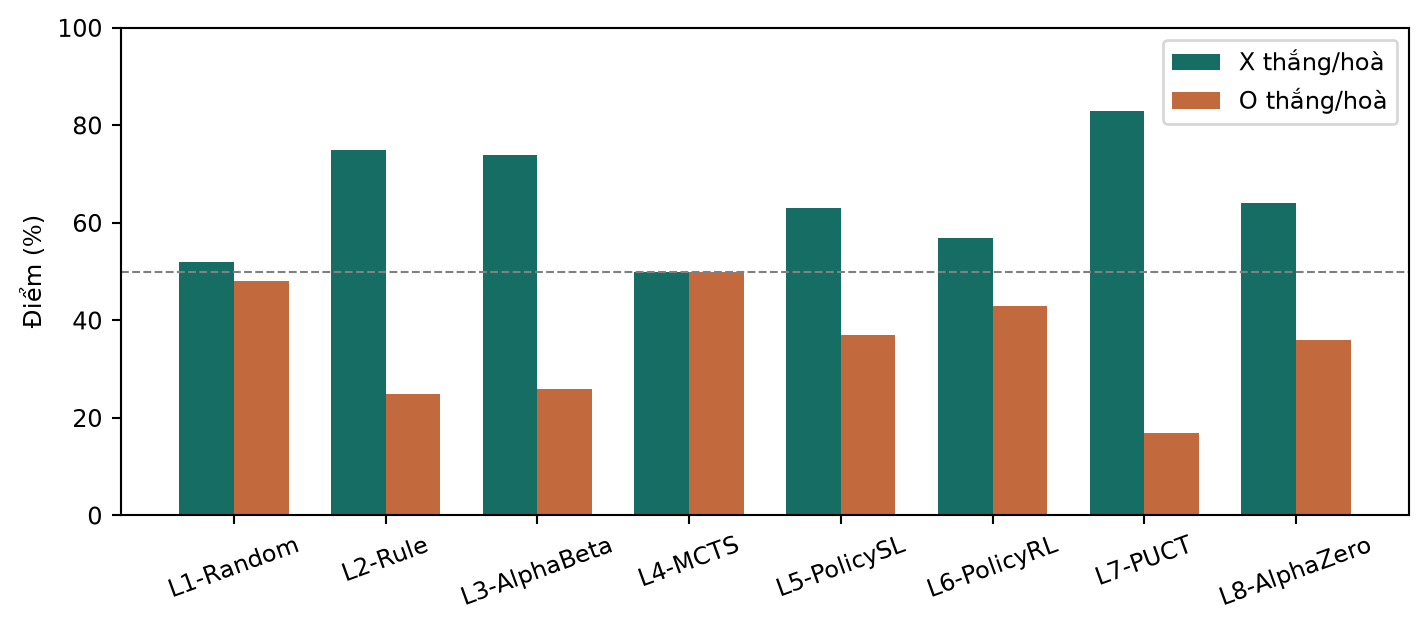
\includegraphics[width=.82\textwidth]{ban-mo-rong/hinh/e3.png}
  \caption{Điểm của bên đi trước (X) và bên đi sau (O) trong tự đấu từng cấp. Điểm tính cả hoà
  nửa điểm. Đường ngang là 50\%.}
  \label{fig:tn-e3}
\end{figure}

\subsection{Kết quả}
Kết quả không đơn điệu theo sức mạnh. L1 Random gần cân bằng (X thắng 52\%, O thắng 48\%), đúng
với kỳ vọng: tác tử ngẫu nhiên không biết khai thác lợi thế đi trước. L2 Rule và L3 Alpha-Beta
lệch mạnh: X thắng 75\% và 66\%, O thắng 25\% và 18\%, còn lại là hoà. L4 MCTS cân bằng tuyệt
đối 50--50. L5 và L6 nằm giữa, với X thắng 62\% và 50\%. Đáng chú ý nhất là cặp PUCT: L7 lệch
mạnh nhất (X thắng 80\%, O thắng 14\%, hoà 6\%), còn L8 — tác tử mạnh hơn — chỉ lệch vừa
(X thắng 50\%, O thắng 22\%, hoà 28\%). L8 tạo ra nhiều ván hoà hơn hẳn, cho thấy nó phòng thủ
tốt hơn khi cầm O và không để thua nhanh.

\subsection{Giải thích}
Có ba cơ chế. Thứ nhất, tác tử tất định có lợi thế đi trước rất rõ nếu chúng có thể tạo đe doạ
bắt buộc sớm: bên X đặt quân trước, kiểm soát trung tâm trước, và buộc bên O phải trả lời. L2
và L3 khai thác được điều này, nên X thắng phần lớn. Thứ hai, MCTS cân bằng vì cả hai bên dùng
cùng một cây tìm kiếm và cùng một chính sách; nếu thuật toán không có tri thức khai cuộc đặc
biệt, nó đối xử với hai màu gần như nhau. Thứ ba, trong cùng họ PUCT, mức lệch không tăng theo sức mạnh: L7 lệch +66 điểm nhưng L8 chỉ
lệch +28 điểm, vì L8 hoà nhiều hơn (28\%). Một tác tử mạnh hơn có thể \emph{giảm} tỷ lệ thắng
quyết định bằng cách phòng thủ tốt hơn, biến nhiều ván thua thành hoà. Vì vậy không thể dùng
chênh lệch X--O làm thước đo sức mạnh; nó đo mức độ ``quyết định'' của cặp đấu.

Kết quả này phản bác một giả định ngây thơ rằng ``lợi thế đi trước là một hằng số của trò
chơi''. Trong thực tế, nó là thuộc tính của \emph{cặp tác tử}: hai tác tử yếu có thể cân bằng,
hai tác tử mạnh có thể lệch, và một tác tử có thể lệch theo hướng này nhưng không lệch theo
hướng khác. Vì vậy RQ4 chỉ có thể trả lời theo từng cấp, không thể gộp thành một con số duy
nhất.

\section{Ablation: cắt tỉa, sắp xếp nước, trọng số lượng giá}
\label{sec:tn-ablation}
\subsection{A1: cắt tỉa Alpha-Beta}
\begin{table}[H]
  \centering\small
  \caption{Benchmark A1/A2/A7: số nút và thời gian trung vị trên tập thế cờ cố định.}
  \label{tab:tn-benchmark}
  \begin{center}\small
\begin{tabular}{@{}llrrrr@{}}
\toprule
Nhóm & Cấu hình & Thế & Nút (P50) & ms (P50) & ms (P95) \\
\midrule
A1 & AB-prune & 50 & 39322 & 1273,1 & 5445,2 \\
A1 & AB-full & 50 & 802217 & 26576,0 & 42474,9 \\
A2 & AB-plain & 10 & 9106 & 990,0 & 993,1 \\
A2 & AB-order & 10 & 372 & 995,1 & 1049,0 \\
A2 & AB-order-tt & 10 & 486 & 994,9 & 1051,2 \\
A7 & AB-default & 10 & 366 & 578,2 & 2760,2 \\
A7 & AB-no-defense & 10 & 580 & 548,7 & 2358,0 \\
\bottomrule
\end{tabular}
\end{center}
\end{table}
A1 so Alpha-Beta độ sâu 3 bật và tắt cắt tỉa, giữ nguyên tập ứng viên và hàm lượng giá. Trên 50
thế cờ, số nút trung vị giảm từ 802\,217 xuống 39\,322, tức khoảng 20,4 lần; thời gian trung vị
giảm từ 26\,576 ms xuống 1\,273 ms, tức khoảng 20,9 lần. Giá trị gốc trùng trên 100\% số thế,
đúng với Định lý~\ref{dl:alpha-beta}. Đây là bằng chứng mạnh nhất về tính đúng đắn của cài đặt
cắt tỉa.

Mức giảm 20 lần nhỏ hơn cận lý thuyết $b^{d/2}$ với $b\approx 70$, vì thứ tự nước trong A1 bị
tắt (\texttt{move\_ordering: false}), nên cắt tỉa chỉ đạt một phần tiềm năng. Đây là thiết kế
có chủ đích: A1 đo riêng tác dụng của cắt tỉa, không trộn với sắp xếp nước. A2 mới đo tác dụng
của sắp xếp.

\subsection{A2: sắp xếp nước và bảng chuyển vị}
A2 chạy ba cấu hình với ngân sách thời gian 1 giây mỗi nước trên 10 thế cờ. Không sắp xếp
(AB-plain) duyệt trung vị 9\,106 nút; có sắp xếp (AB-order) chỉ duyệt 372 nút, giảm khoảng 24,5
lần; thêm bảng chuyển vị (AB-order-tt) duyệt 486 nút. Thời gian trung vị gần nhau (990--995
ms) vì cả ba đều dừng theo ngân sách 1 giây. Kết quả này cho thấy sắp xếp nước giúp \emph{đi
sâu hơn trong cùng thời gian}, chứ không nhất thiết giúp \emph{chạy nhanh hơn}. Muốn đo tăng
tốc, phải cố định độ sâu; muốn đo chất lượng, phải đo độ sâu đạt được hoặc điểm đấu.

AB-order-tt duyệt nhiều nút hơn AB-order một chút. Điều này không có nghĩa TT làm chậm; nó có
thể do TT cho phép tìm sâu hơn trong cùng 1 giây, nên số nút tăng. Log benchmark không ghi độ
sâu đạt được, nên không thể tách hai khả năng. Đây là một giới hạn của phép đo A2, được ghi ở
Mục~\ref{sec:tn-han-che}.

\subsection{A7: trọng số hàm lượng giá}
A7 so hai bảng trọng số: mặc định (tính cả tấn công và phòng thủ) và \texttt{no\_defense} (chỉ
tính quân mình). Trên 10 thế cờ, giá trị gốc chỉ trùng trên 1/10 thế, tức 10\%. Số nút trung
vị là 366 (mặc định) và 580 (bỏ phòng thủ). Kết quả này xác nhận rằng thành phần phòng thủ
trong hàm lượng giá thay đổi quyết định chọn nước, không chỉ thay đổi điểm số. Tuy nhiên, nó
không cho biết bảng nào chơi mạnh hơn; muốn biết phải đấu trực tiếp. A7b (nếu có) trả lời câu
hỏi đó.

\subsection{A8: chiến thuật tại gốc}
A8 so MCTS rollout nhẹ có và không có \texttt{root\_tactics}. Kết quả A3/A4 cho thấy MCTS bỏ
chặn rất nhiều, nên giả thuyết là bật chiến thuật tại gốc sẽ cải thiện mạnh. Tuy nhiên, bản
tiến độ chỉ có cấu hình, chưa có kết quả đối đầu đủ lớn. A8b được thiết kế để lấp khoảng trống
này; nếu chưa chạy xong, mục này ghi rõ là chưa kết luận được.

\subsection{A6: tăng cường đối xứng}
A6 so huấn luyện có và không có tăng cường D4. Bản tiến độ mới có cấu hình, chưa có cặp
checkpoint tương ứng. Đây là phần cần bổ sung: huấn luyện hai mô hình cùng dữ liệu, cùng epoch,
khác cờ \texttt{augment\_x8}, rồi đấu trên cùng tập khai cuộc. Báo cáo không suy đoán kết quả
từ lý thuyết, vì tăng cường đối xứng có thể giúp ích hoặc không tuỳ dữ liệu.

\section{MCTS thuần: số mô phỏng và rollout}
\label{sec:tn-mcts}
\subsection{A3: số mô phỏng}
\begin{table}[H]
  \centering\small
  \caption{A3/A4: điểm, thời gian mỗi nước và tốc độ mô phỏng của MCTS trước L2 và L3. Mỗi ô
  có 200 ván.}
  \label{tab:tn-a3a4}
  \begin{center}\small
\begin{tabular}{@{}llrrrrrrr@{}}
\toprule
Mã & Cấu hình & Gặp & Ván & W/D/L & Điểm & ms P50 & ms P95 & mp/s \\
\midrule
A3 & MCTS-100 & L2 & 200 & 0/0/200 & 0,0\% & 15,8 & 26,5 & 5951 \\
A3 & MCTS-100 & L3 & 200 & 0/0/200 & 0,0\% & 16,4 & 19,9 & 6262 \\
A3 & MCTS-1600 & L2 & 200 & 0/0/200 & 0,0\% & 307,3 & 370,7 & 5284 \\
A3 & MCTS-1600 & L3 & 200 & 0/0/200 & 0,0\% & 302,9 & 353,4 & 5432 \\
A3 & MCTS-400 & L2 & 200 & 0/0/200 & 0,0\% & 68,8 & 79,7 & 6014 \\
A3 & MCTS-400 & L3 & 200 & 0/0/200 & 0,0\% & 72,0 & 89,4 & 5632 \\
A3 & MCTS-6400 & L2 & 200 & 15/0/185 & 7,5\% & 1225,5 & 1471,7 & 5322 \\
A3 & MCTS-6400 & L3 & 200 & 4/0/196 & 2,0\% & 1244,5 & 1461,0 & 5301 \\
A4 & MCTS-light & L2 & 200 & 0/0/200 & 0,0\% & 625,3 & 735,7 & 1407 \\
A4 & MCTS-light & L3 & 200 & 0/0/200 & 0,0\% & 611,5 & 752,9 & 1485 \\
A4 & MCTS-random & L2 & 200 & 0/0/200 & 0,0\% & 150,6 & 188,3 & 5413 \\
A4 & MCTS-random & L3 & 200 & 0/0/200 & 0,0\% & 151,8 & 176,6 & 5454 \\
\bottomrule
\end{tabular}
\end{center}
\end{table}
A3 cho MCTS rollout ngẫu nhiên đấu L2 và L3 ở bốn mức 100, 400, 1\,600 và 6\,400 mô phỏng.
Ở ba mức đầu, MCTS thua toàn bộ 200 ván trước mỗi đối thủ. Ở 6\,400 mô phỏng, MCTS thắng 15/200
trước L2 (7,5\%) và 4/200 trước L3 (2,0\%). Thời gian mỗi nước tăng gần tuyến tính theo số mô
phỏng: khoảng 16 ms ở 100, 69 ms ở 400, 307 ms ở 1\,600 và 1\,225 ms ở 6\,400. Tốc độ khoảng
5\,300--6\,000 mô phỏng/giây, giảm nhẹ khi cây lớn hơn.

Điểm tăng từ 0 lên 7,5\% khi tăng 16 lần số mô phỏng là một cải thiện rất nhỏ so với chi phí.
Điều này khớp với giả thuyết ở Mục~\ref{sec:lt-vcf}: MCTS cần đủ độ sâu để thấy chuỗi ép 4 ply,
nhưng với 40--70 nước gốc, 6\,400 mô phỏng chỉ cho mỗi nước khoảng 90--160 lượt thăm, chưa đủ
để phân biệt nhánh thắng và nhánh thua trong một chuỗi dài. Rollout ngẫu nhiên càng làm nhiễu
giá trị: kết quả mô phỏng không phản ánh chất lượng nước gốc.

\subsection{A4: kiểu rollout}
A4 giữ 800 mô phỏng và đổi rollout giữa \texttt{random} và \texttt{light}. Cả hai đều thua
toàn bộ 400 ván trước L2 và L3, nên \emph{không phân biệt được hai kiểu rollout qua điểm số}.
Hai kiểu khác nhau rõ về chi phí: rollout ngẫu nhiên mất khoảng 151 ms/nước, rollout nhẹ mất
khoảng 615--625 ms/nước, tức chậm khoảng 4 lần. Rollout nhẹ tốn thời gian vì mỗi bước phải gọi
\texttt{winning\_squares} cho cả hai bên, nhưng không đủ để bù khoảng cách chiến thuật ở gốc.

\subsection{Phân loại lỗi}
Bảng~\ref{tab:tn-loi-mcts} phân loại lỗi trong các ván MCTS thua, dùng script
\repoFile{report/scripts/phan\_tich\_loi\_mcts.py}. Tại nước cuối của MCTS, nếu đối thủ có đúng
một ô thắng và MCTS không chặn, đó là ``bỏ sót chặn năm''. Nếu đối thủ đã có từ hai ô thắng,
ván đã thua; script xét nước kế cuối và tìm nước của đối thủ tạo từ hai ô thắng mà MCTS không
ngăn (``bỏ sót chặn ba hở / đòn kép'').

\begin{table}[H]
  \centering\small
  \caption{Phân loại lỗi trong các ván MCTS thua ở A3/A4. Tỷ lệ tính trên số ván thua của cấu
  hình.}
  \label{tab:tn-loi-mcts}
  \begin{tabular}{@{}lrrr@{}}
    \toprule
    \textbf{Cấu hình} & \textbf{Ván thua} & \textbf{Bỏ sót đe doạ kép} & \textbf{Bỏ sót chặn năm} \\
    \midrule
    A3, 100 mô phỏng & 400 & 92,5\% & 7,5\% \\
    A3, 400 mô phỏng & 400 & 91,2\% & 8,8\% \\
    A3, 1\,600 mô phỏng & 400 & 88,5\% & 11,5\% \\
    A3, 6\,400 mô phỏng & 381 & 92,9\% & 7,1\% \\
    A4, rollout ngẫu nhiên & 400 & 89,8\% & 10,2\% \\
    A4, rollout nhẹ & 400 & 65,2\% & 34,8\% \\
    \bottomrule
  \end{tabular}
\end{table}

Hai nhận xét. Thứ nhất, lỗi chủ đạo ở mọi mức mô phỏng là không ngăn đe doạ kép sớm (khoảng
90\%); tăng mô phỏng từ 100 lên 6\,400 không đổi tỷ lệ này. Điều này khớp với giả thuyết cây
quá nông cho cấu trúc 4 ply. Thứ hai, rollout nhẹ làm tỷ lệ bỏ sót chặn năm \emph{tăng} lên
34,8\%, dù rollout đã biết chặn. Nguyên nhân là rollout chỉ chặn bên trong mô phỏng, còn ở gốc
cây thống kê thăm quá thưa nên nước chặn bắt buộc có thể không được chọn. Đây là một phản ví
dụ thú vị: cải thiện rollout không tự động cải thiện quyết định ở gốc.

\section{Policy-only, PUCT và cùng mạng}
\label{sec:tn-a5}
\begin{table}[H]
  \centering\small
  \caption{A5: policy-only, PUCT và các mốc mô phỏng. Mỗi dòng 200 ván; khoảng tin cậy Wilson
  95\%.}
  \label{tab:tn-a5}
  \begin{center}\small
\begin{tabular}{@{}llrrrr@{}}
\toprule
Tác tử & Đối thủ & Ván & W/D/L & Điểm & Wilson 95\% \\
\midrule
l5\_policy\_sl & l2\_rule & 200 & 130/2/68 & 65,50\% & [58,7\%; 71,7\%] \\
l5\_policy\_sl & l3\_alphabeta & 200 & 41/2/157 & 21,00\% & [15,9\%; 27,2\%] \\
l6\_policy\_rl & l2\_rule & 200 & 151/5/44 & 76,75\% & [70,4\%; 82,1\%] \\
l6\_policy\_rl & l3\_alphabeta & 200 & 54/19/127 & 31,75\% & [25,7\%; 38,5\%] \\
L7-PUCT[l5,100] & l3\_alphabeta & 200 & 88/9/103 & 46,25\% & [39,5\%; 53,2\%] \\
L7-PUCT[l5,200] & l3\_alphabeta & 200 & 104/26/70 & 58,50\% & [51,6\%; 65,1\%] \\
L7-PUCT[l5,400] & l3\_alphabeta & 200 & 105/34/61 & 61,00\% & [54,1\%; 67,5\%] \\
L7-PUCT[l5,800] & l3\_alphabeta & 200 & 118/32/50 & 67,00\% & [60,2\%; 73,1\%] \\
L7-PUCT[l5,200] & l2\_rule & 200 & 175/1/24 & 87,75\% & [82,5\%; 91,6\%] \\
L7-PUCT[l6,200] & l3\_alphabeta & 200 & 105/21/74 & 57,75\% & [50,8\%; 64,4\%] \\
L7-PUCT[l5,200] & l5\_policy\_sl & 200 & 191/0/9 & 95,50\% & [91,7\%; 97,6\%] \\
\bottomrule
\end{tabular}
\end{center}
\end{table}
A5 giữ cùng một mạng và thay đổi cách dùng nó. Kết quả chính:
\begin{itemize}
  \item L5 policy-only đạt 21,0\% trước L3; L6 đạt 31,75\%.
  \item L7 PUCT dùng mạng L5 đạt 46,25\% ở 100 mô phỏng, 58,5\% ở 200, 61,0\% ở 400 và 67,0\%
        ở 800, đều trước L3.
  \item L7 ở 200 mô phỏng thắng L5 191/200 ván (95,5\%).
  \item L7 dùng mạng L5 và mạng L6 chênh nhau 0,75 điểm phần trăm trước L3 ở 200 mô phỏng.
\end{itemize}
So sánh cùng mạng là điểm mạnh của A5: nó tách đóng góp của \emph{tìm kiếm} khỏi đóng góp của
\emph{trọng số}. Với cùng mạng L5, thêm PUCT làm điểm trước L3 tăng từ 21,0\% lên 58,5\%, tức
37,5 điểm phần trăm. Đây là bằng chứng mạnh rằng tìm kiếm bù được một phần điểm yếu của policy
học bắt chước.

Tuy nhiên, khoảng tin cậy của 200 và 800 mô phỏng chồng lấn (58,5\% [51,6; 65,1] so với 67,0\%
[60,2; 73,1]), nên chưa thể khẳng định 800 mô phỏng tốt hơn 200 một cách chắc chắn. Xu hướng
tăng là rõ, nhưng mức tăng 8,5 điểm nằm trong sai số. Tương tự, chênh lệch 0,75 điểm giữa hai
mạng nhỏ hơn nhiều so với khoảng tin cậy, nên không xếp hạng được hai mạng trong PUCT.

\section{Học có giám sát: policy, value và lỗi quy ước}
\label{sec:tn-sl}
\begin{table}[H]
  \centering\small
  \caption{Chỉ số huấn luyện và đối đầu của các checkpoint SL/RL (nguồn: \texttt{runs/train}).}
  \label{tab:tn-hoc}
  \begin{center}\small
\begin{tabular}{@{}lrrrr@{}}
\toprule
Mạng & Số epoch & Epoch tốt nhất & Val loss tốt nhất & Val loss cuối \\
\midrule
SL v1 & 30 & 30 & 2,1566 & 2,1566 \\
SL v2 & 30 & 28 & 1,6020 & 1,7095 \\
SL v3 & 60 & 55 & 1,4723 & 1,4758 \\
\bottomrule
\end{tabular}
\end{center}
\begin{center}\small
\begin{tabular}{@{}llrrr@{}}
\toprule
Checkpoint & Đối thủ & Ván & W/D/L & Điểm \\
\midrule
SL v1 & L2 & 100 & 40/0/60 & 40,0\% \\
SL v1 & L3 & 100 & 5/0/95 & 5,0\% \\
SL v2 & L2 & 100 & 66/0/34 & 66,0\% \\
SL v2 & L3 & 100 & 19/3/78 & 20,5\% \\
SL v3 & L2 & 100 & 63/6/31 & 66,0\% \\
SL v3 & L3 & 100 & 19/4/77 & 21,0\% \\
RL v2 best & L2 & 100 & 72/1/27 & 72,5\% \\
RL v2 best & L3 & 100 & 25/5/70 & 27,5\% \\
RL v3 best & L2 & 100 & 79/4/17 & 81,0\% \\
RL v3 best & L3 & 100 & 33/8/59 & 37,0\% \\
RL v3 last & L2 & 100 & 81/1/18 & 81,5\% \\
RL v3 last & L3 & 100 & 33/7/60 & 36,5\% \\
\bottomrule
\end{tabular}
\end{center}
\end{table}
\begin{table}[H]
  \centering\small
  \caption{Top-1/top-3 policy và calibration value trên tập test \texttt{expert\_v2}.}
  \label{tab:tn-hoc-moi}
  \begin{center}\small
\begin{tabular}{@{}lrrrrrr@{}}
\toprule
Mạng & Top-1 & Top-3 & CE policy & MSE value & Tương quan & Đúng dấu \\
\midrule
SL v1 & 44,0\% & 71,2\% & 2,373 & 1,441 & -0,012 & 45,7\% \\
SL v2 & 65,3\% & 89,3\% & 1,143 & 1,377 & +0,005 & 45,8\% \\
SL v3 & 67,8\% & 89,4\% & 1,009 & 0,356 & +0,778 & 77,6\% \\
\bottomrule
\end{tabular}
\end{center}
\begin{center}\small
\begin{tabular}{@{}lrrrrrr@{}}
\toprule
Mạng & MSE đầu & MSE giữa & MSE cuối & r đầu & r giữa & r cuối \\
\midrule
SL v1 & 1,431 & 1,388 & 1,497 & -0,021 & +0,016 & -0,021 \\
SL v2 & 1,174 & 1,313 & 1,631 & +0,015 & +0,005 & -0,001 \\
SL v3 & 0,635 & 0,362 & 0,083 & +0,552 & +0,774 & +0,953 \\
\bottomrule
\end{tabular}
\end{center}
\end{table}
\subsection{Độ chính xác policy}
Trên tập test tách theo ván của \texttt{expert\_v2} (29\,161 mẫu, 1\,883 ván), SL v1 đạt top-1
44,0\% và top-3 71,2\%; SL v2 đạt 65,3\% và 89,3\%; SL v3 đạt 67,8\% và 89,4\%. Sự nhảy vọt từ
v1 sang v2 đến từ dữ liệu: v1 dùng 27\,720 mẫu với temperature 0,5 và top-k 3, gần như luôn
chọn nước tốt nhất; v2 dùng 297\,098 mẫu với temperature 8,0 và top-k 5, đa dạng hơn nhiều.
Mạng học được nhiều tình huống hơn, nên top-1 tăng 21 điểm phần trăm.

Từ v2 sang v3, top-1 chỉ tăng 2,5 điểm, dù v3 huấn luyện 60 epoch thay vì 30 và dùng cosine
learning rate. Điều này cho thấy trần của việc bắt chước Alpha-Beta độ sâu 3 đã gần đạt: thêm
epoch không tạo thêm thông tin. Muốn vượt trần, phải đổi nguồn nhãn (RL hoặc self-play) hoặc
tăng chất lượng chuyên gia.

\subsection{Value head và lỗi quy ước dấu}
Bảng~\ref{tab:tn-value} tóm tắt calibration của value head. SL v1 và v2 được huấn luyện với
nhãn \emph{tuyệt đối} (+1 nếu X thắng), trong khi đầu vào mạng và RL cần nhãn \emph{theo góc
nhìn người đi}. Vì vậy, khi đánh giá theo nhãn người đi, MSE của v1/v2 cao (1,44 và 1,38) và
tương quan gần 0; tách theo màu cho thấy tương quan +0,73 ở thế X đi nhưng −0,73 ở thế O đi.
Đây là dấu hiệu kinh điển của lỗi đảo dấu ở một nửa số thế.

SL v3 sửa lỗi bằng cách đổi nhãn ngay khi nạp dữ liệu. Kết quả: MSE giảm còn 0,356, tương quan
+0,778, độ chính xác dấu 77,6\%, và đối xứng giữa X đi và O đi (0,355/0,358; +0,770/+0,774).
Tách theo giai đoạn ván, MSE giảm từ 0,635 ở đầu ván xuống 0,362 ở giữa và 0,083 ở cuối ván;
tương quan tăng từ +0,552 lên +0,774 và +0,953. Điều này hợp lý: cuối ván, kết quả gần như đã
định đoạt nên value dễ dự đoán; đầu ván, có nhiều nhánh và value khó hơn.

\begin{table}[H]
  \centering\small
  \caption{Calibration của value head trên tập test \texttt{expert\_v2}. ``Nhãn người đi'' là
  quy ước đúng cho RL/PUCT; ``nhãn tuyệt đối'' là quy ước dùng khi sinh dữ liệu.}
  \label{tab:tn-value}
  \begin{tabular}{@{}lrrrrrr@{}}
    \toprule
    \textbf{Mạng} & \textbf{MSE (người đi)} & \textbf{Tương quan} & \textbf{Đúng dấu} &
    \textbf{MSE (tuyệt đối)} & \textbf{r (X đi)} & \textbf{r (O đi)} \\
    \midrule
    SL v1 & 1,441 & −0,012 & 45,7\% & 0,846 & +0,390 & −0,415 \\
    SL v2 & 1,377 & +0,005 & 45,8\% & 0,418 & +0,730 & −0,729 \\
    SL v3 & 0,356 & +0,778 & 77,6\% & 1,451 & +0,770 & +0,774 \\
    \bottomrule
  \end{tabular}
\end{table}

\begin{figure}[H]
  \centering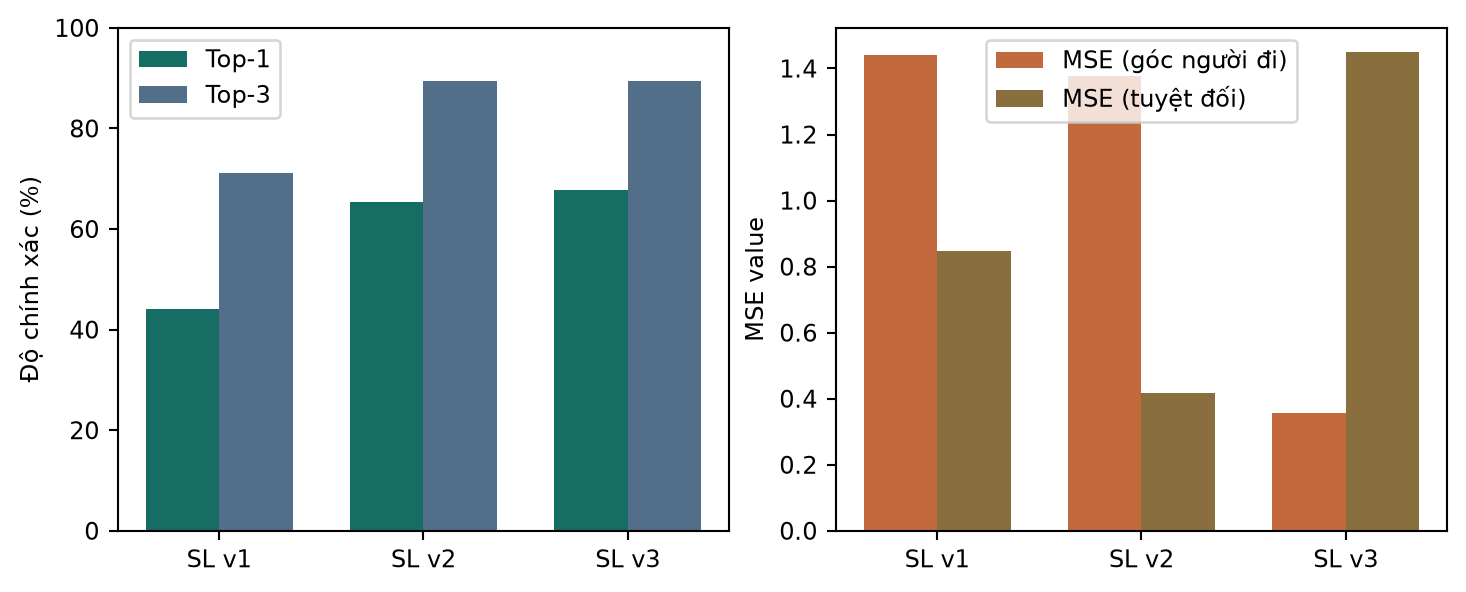
\includegraphics[width=.9\textwidth]{ban-mo-rong/hinh/hoc-moi.png}
  \caption{Trái: top-1/top-3 policy trên tập test. Phải: MSE value theo hai quy ước nhãn. SL v3
  là bản đã sửa quy ước; MSE theo nhãn người đi thấp hơn hẳn, còn MSE theo nhãn tuyệt đối cao
  hơn vì mạng không còn học quy ước đó.}
  \label{fig:tn-hoc}
\end{figure}

\subsection{Entropy policy}
Entropy trung bình của policy dự đoán là 1,69 (v1), 1,13 (v2) và 1,01 (v3), trong khi entropy
của nhãn là 0,618. Mạng vẫn ``bảo thủ'' hơn nhãn: nó phân bố xác suất rộng hơn phân phối mục
tiêu. Điều này có thể do temperature của dữ liệu và do mạng chưa đủ dung lượng/thời gian để học
các phân phối sắc. Với PUCT, policy quá mềm không nhất thiết xấu, vì tìm kiếm sẽ điều chỉnh;
nhưng với policy-only, phân phối mềm làm argmax kém ổn định.

\section{Học tăng cường}
\label{sec:tn-rl}
\begin{table}[H]
  \centering\small
  \caption{Các mốc đánh giá của REINFORCE v2/v3 (100 ván mỗi đối thủ mỗi mốc).}
  \label{tab:tn-l6}
  \begin{center}\small
\begin{tabular}{@{}lrrr@{}}
\toprule
Mạng & Episode & Điểm gặp L2 & Điểm gặp L3 \\
\midrule
RL v2 & 5120 & 61,5\% & 18,0\% \\
RL v2 & 10112 & 50,5\% & 14,5\% \\
RL v2 & 15104 & 57,0\% & 23,5\% \\
RL v2 & 20096 & 70,0\% & 19,5\% \\
RL v2 & 25088 & 73,5\% & 22,0\% \\
RL v2 & 30080 & 68,0\% & 26,5\% \\
RL v2 & 35072 & 74,0\% & 30,5\% \\
RL v2 & 40064 & 73,5\% & 29,5\% \\
RL v2 & 45056 & 74,0\% & 23,5\% \\
RL v2 & 49920 & 72,5\% & 29,5\% \\
RL v3 & 5120 & 53,5\% & 19,0\% \\
RL v3 & 10112 & 74,0\% & 17,5\% \\
RL v3 & 15104 & 69,5\% & 18,0\% \\
RL v3 & 20096 & 76,5\% & 31,0\% \\
RL v3 & 25088 & 78,0\% & 30,0\% \\
RL v3 & 30080 & 70,5\% & 31,0\% \\
RL v3 & 35072 & 80,0\% & 35,5\% \\
RL v3 & 40064 & 74,5\% & 30,5\% \\
RL v3 & 45056 & 78,0\% & 33,0\% \\
RL v3 & 49920 & 78,5\% & 26,0\% \\
\bottomrule
\end{tabular}
\end{center}
\end{table}
\begin{figure}[H]
  \centering
  \begin{subfigure}[t]{.49\textwidth}\centering
    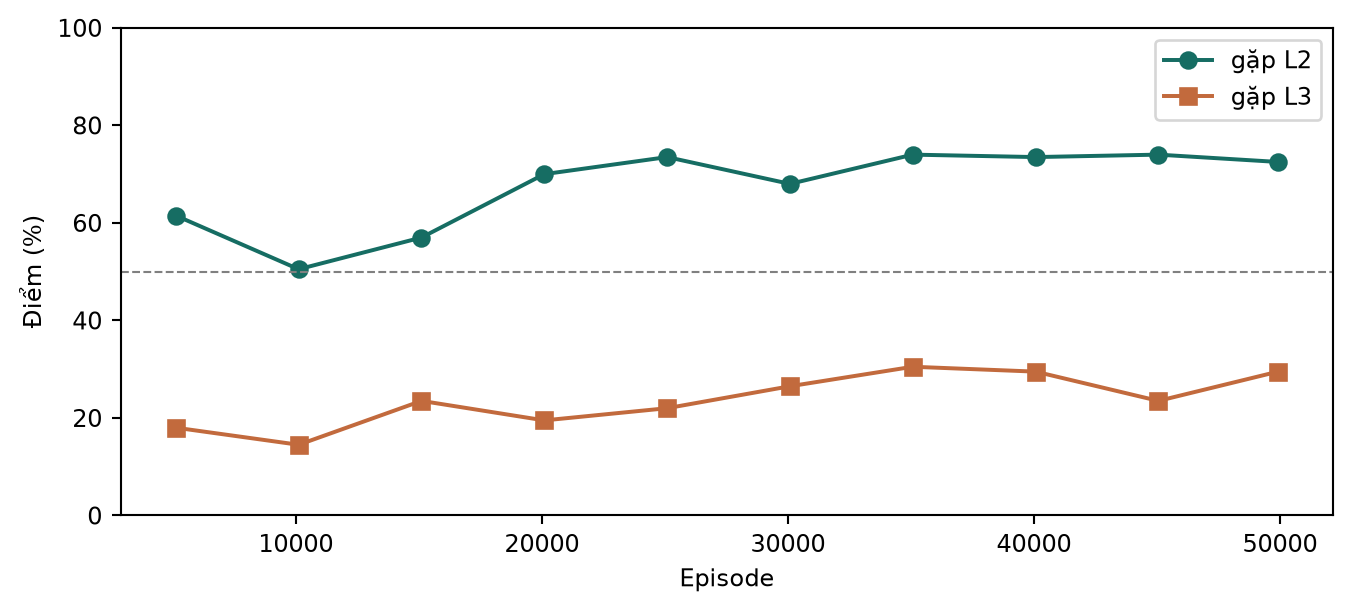
\includegraphics[width=\textwidth]{ban-mo-rong/hinh/l6-RLv2.png}
    \caption{RL v2 khởi tạo từ SL v2.}
  \end{subfigure}\hfill
  \begin{subfigure}[t]{.49\textwidth}\centering
    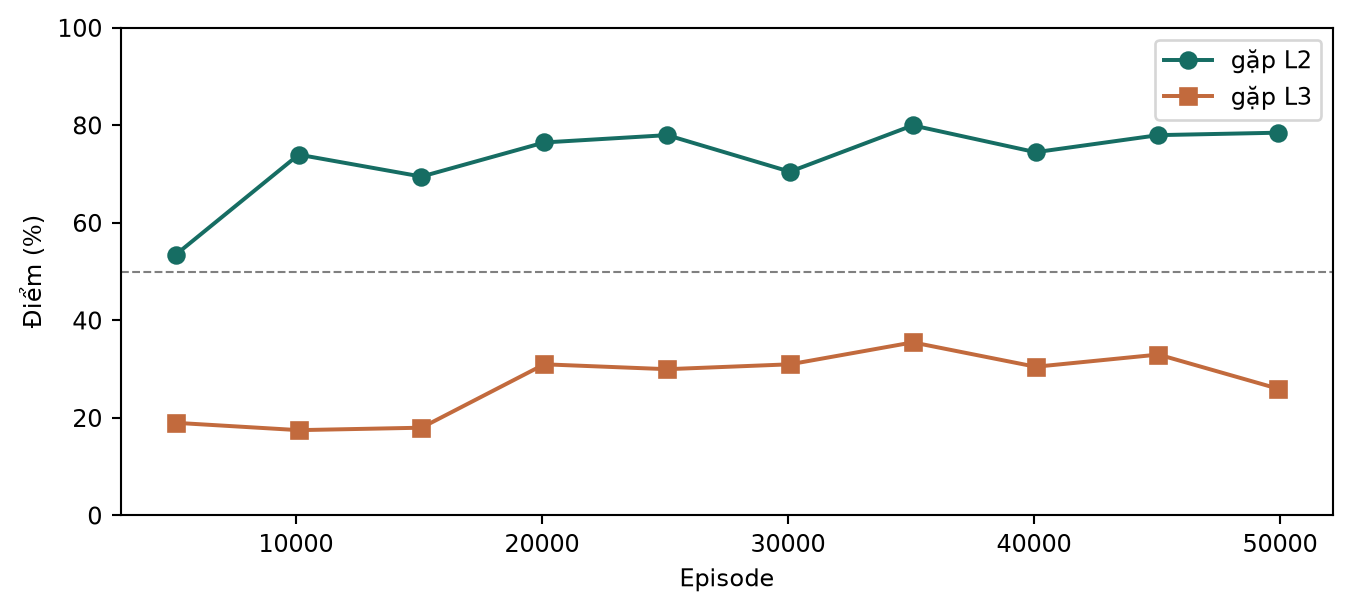
\includegraphics[width=\textwidth]{ban-mo-rong/hinh/l6-RLv3.png}
    \caption{RL v3 khởi tạo từ SL v3.}
  \end{subfigure}
  \caption{Đường cong đánh giá của REINFORCE qua 10 mốc, mỗi mốc 100 ván trước L2 và L3.}
  \label{fig:tn-l6}
\end{figure}

RL v3 chạy 49\,920 episode, hơn 1,5 triệu nước, với 10 mốc đánh giá. Điểm trước L2 dao động
53,5--80,0\%, trước L3 dao động 17,5--35,5\%. Điểm cuối là 78,5\% trước L2 và 26,0\% trước L3.
So với SL v3 (66,0\% trước L2, 21,0\% trước L3 trong phép đánh giá checkpoint), RL v3 cải thiện
khoảng 12--16 điểm phần trăm. Đây là bằng chứng định lượng cho RQ2: self-play có cải thiện so
với bắt chước, nhưng mức cải thiện không đồng đều và có dao động.

Dao động giữa các mốc có hai nguồn. Thứ nhất, trọng số thay đổi qua các vòng. Thứ hai, mỗi mốc
dùng một bộ khai cuộc sinh từ seed khác nhau, nên so sánh giữa các mốc không phải so sánh trên
cùng tập thế. Vì vậy đường cong nên đọc như xu hướng, không như một chuỗi đo lường chính xác.
Điểm cao nhất trước cả hai đối thủ rơi vào episode 35\,072, sau đó giảm; điều này có thể do
quá khớp hoặc do nhiễu khai cuộc. Chọn checkpoint theo tiêu chí định trước và đánh lại trên tập
giữ riêng sẽ phân biệt hai khả năng; báo cáo chưa làm được vì thiếu thời gian.

\section{Vòng lặp AlphaZero}
\label{sec:tn-l8}
\begin{table}[H]
  \centering\small
  \caption{Các vòng L8 được duyệt qua gating (100 ván mỗi vòng, ngưỡng 55\%).}
  \label{tab:tn-l8}
  \begin{center}\small
\begin{tabular}{@{}lrrr@{}}
\toprule
Vòng duyệt & Ván & W/D/L & Điểm \\
\midrule
12 & 100 & 56/3/41 & 57,5\% \\
18 & 100 & 54/10/36 & 59,0\% \\
19 & 100 & 49/13/38 & 55,5\% \\
24 & 100 & 49/12/39 & 55,0\% \\
29 & 100 & 55/14/31 & 62,0\% \\
37 & 100 & 53/16/31 & 61,0\% \\
\bottomrule
\end{tabular}
\end{center}
\end{table}
\begin{figure}[H]
  \centering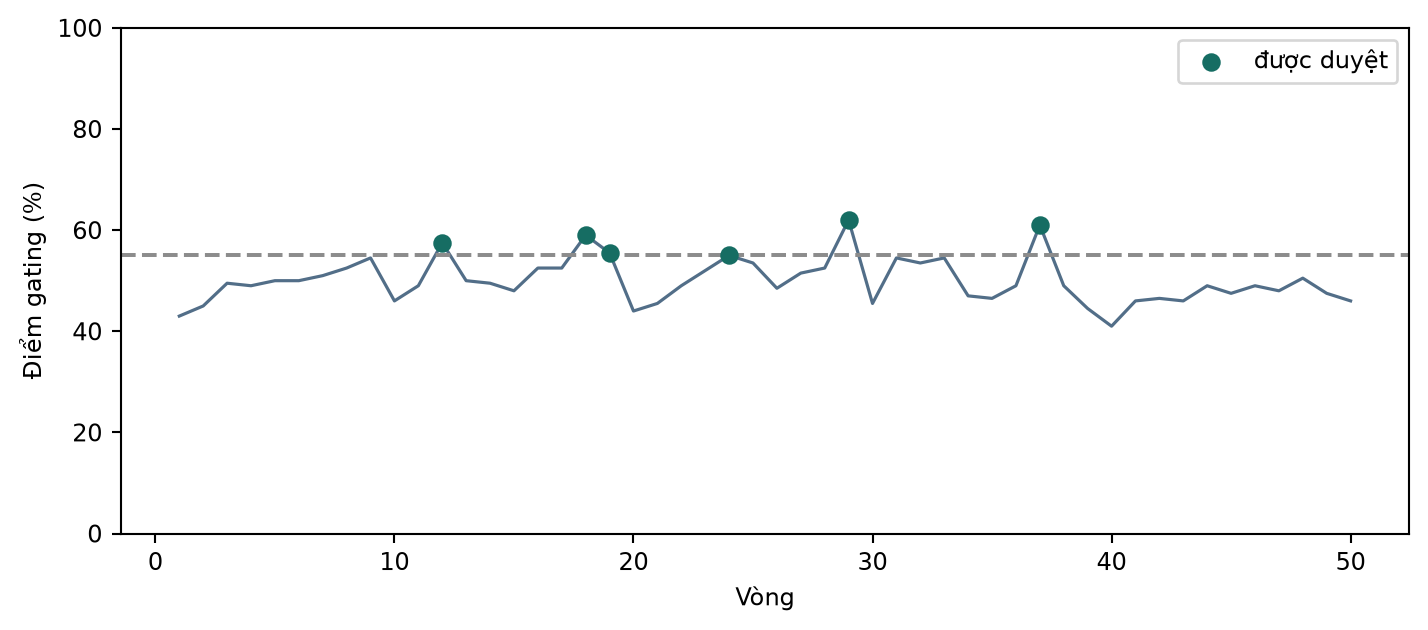
\includegraphics[width=.9\textwidth]{ban-mo-rong/hinh/l8-moi.png}
  \caption{Điểm gating qua 50 vòng. Điểm là tỷ lệ của ứng viên trước bản đương nhiệm tại thời
  điểm đó; ngưỡng duyệt 55\%. Các điểm tròn là vòng được duyệt.}
  \label{fig:tn-l8}
\end{figure}

L8 chạy 50 vòng, mỗi vòng 200 ván tự đấu ở 400 mô phỏng, 1\,000 bước cập nhật, và 100 ván
gating ở 200 mô phỏng. Tổng cộng 10\,000 ván tự đấu trong khoảng 12 giờ 19 phút trên GPU. Ứng
viên được duyệt ở các vòng 12, 18, 19, 24, 29 và 37; vòng 37 là lần duyệt cuối và là
checkpoint \texttt{best.pt}. Điểm gating của các vòng được duyệt lần lượt 57,5\%, 59,0\%,
55,5\%, 55,0\%, 62,0\% và 61,0\%.

Cần đọc điểm gating đúng cách: mỗi vòng so ứng viên với \emph{bản đương nhiệm tại thời điểm
đó}, không phải với một đối thủ cố định. Vì vậy không thể so 62,0\% của vòng 29 với 61,0\% của
vòng 37 để nói vòng 29 tốt hơn. Điểm gating chỉ trả lời câu hỏi ``ứng viên có đủ tốt để thay
bản hiện tại không'', không trả lời ``ứng viên mạnh đến đâu''. Muốn trả lời câu thứ hai, cần
đấu với đối thủ cố định, như phép đấu cuối với L7 và L3.

Kết quả cuối: L8 best thắng L7 16/20 ván (82,5\%, 1 hoà) và thắng L3 25/40 ván (68,75\%,
5 hoà). Theo màu, L8 cầm X đạt 90,0\% trước L7 và 92,5\% trước L3; cầm O đạt 75,0\% và 45,0\%.
Chênh lệch theo màu rất lớn, đặc biệt trước L3 (47,5 điểm phần trăm), cho thấy L8 vẫn phụ thuộc
vào lợi thế đi trước. Cỡ mẫu 20 và 40 ván nhỏ; khoảng bootstrap 95\% của L8 trước L3 là
60,0--77,5\%, nên mức 68,75\% là ước lượng trung bình, không phải một con số chính xác.

\subsection{Tự đấu từ bàn trống và tự đấu từ khai cuộc}
\label{sec:tn-l8-selfplay}
Mười nghìn ván tự đấu của L8 bắt đầu từ bàn trống, không dùng khai cuộc. Kết quả: X thắng
7\,701 ván (77,0\%), O thắng 923 ván (9,2\%), hoà 1\,376 ván (13,8\%). Điểm của X là 83,9\%.
Độ dài trung bình 34,9 nước, trung vị 22, p95 121. Tỷ lệ này cao hơn nhiều so với E3 của L8
(X 50\%, O 22\%, hoà 28\%, điểm X 64\%). Hình~\ref{fig:tn-l8-color} cho thấy tỷ lệ không đổi
nhiều qua bốn phần của quá trình huấn luyện: X luôn thắng khoảng 70--80\%.

\begin{figure}[H]
  \centering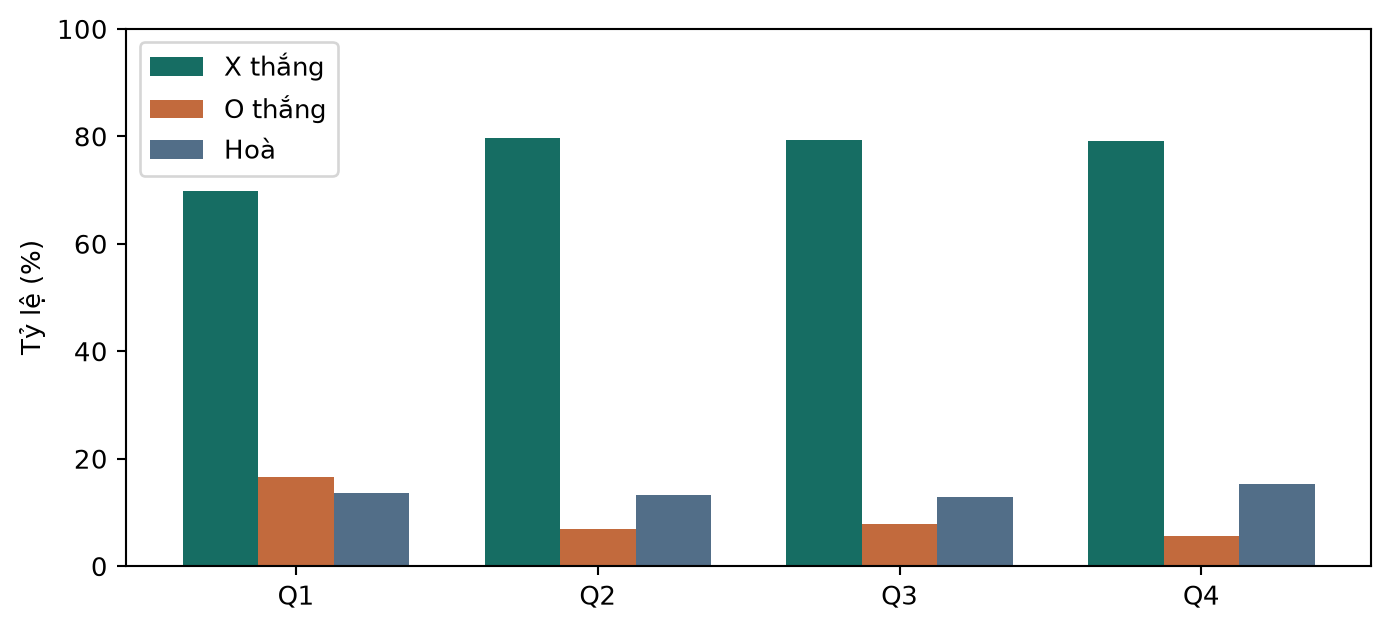
\includegraphics[width=.82\textwidth]{ban-mo-rong/hinh/l8-selfplay-color.png}
  \caption{Tỷ lệ X thắng/O thắng/hoà trong 10\,000 ván tự đấu của L8, chia bốn phần theo thời
  gian. Tự đấu bắt đầu từ bàn trống và dùng nhiễu Dirichlet.}
  \label{fig:tn-l8-color}
\end{figure}

Có bốn khác biệt giữa hai phép đo, không thể quy toàn bộ chênh lệch cho một yếu tố:
\begin{enumerate}
  \item \textbf{Khai cuộc:} tự đấu bắt đầu từ bàn trống; E3 bắt đầu từ 2--4 nước ngẫu nhiên
        trong vùng trung tâm. Khai cuộc làm giảm lợi thế đi trước vì nó phá thế đối xứng và tạo
        ra nhiều thế cờ khác nhau.
  \item \textbf{Số mô phỏng:} tự đấu dùng 400 mô phỏng; E3 dùng 200. Nhiều mô phỏng hơn giúp
        bên đi trước khai thác lợi thế tốt hơn, nhưng cũng giúp bên đi sau phòng thủ tốt hơn;
        chiều tác động không rõ.
  \item \textbf{Nhiễu và nhiệt độ:} tự đấu dùng Dirichlet $\alpha=0{,}3$, $\varepsilon=0{,}25$
        và temperature 1 cho 8 nước đầu; E3 không dùng. Nhiễu làm đa dạng khai cuộc, có thể
        giảm lợi thế của X nếu nó đẩy X ra khỏi nước tốt nhất.
  \item \textbf{Thực thể:} tự đấu dùng cùng một mạng cho cả hai bên; E3 dùng hai thực thể độc
        lập cùng trọng số. Khác biệt này nhỏ vì trọng số giống nhau, nhưng RNG khác nhau.
\end{enumerate}

Điểm quan trọng nhất là \emph{khai cuộc làm giảm mạnh lợi thế đi trước}. Đây là bằng chứng
định lượng cho quyết định dùng 50 khai cuộc đổi màu trong mọi giải đấu: nếu đánh từ bàn trống,
kết quả sẽ bị chi phối bởi lợi thế X, không phải bởi sức mạnh tác tử. Nó cũng cảnh báo về việc
huấn luyện tự đấu từ bàn trống: mạng có thể học quá nhiều dòng X thắng và ít dòng O phòng thủ
thành công. Trong tương lai, nên trộn khai cuộc ngẫu nhiên vào tự đấu để cân bằng dữ liệu.

Gating cũng cho thấy lợi thế màu: trong 5\,000 ván gating, X thắng 3\,018 (60,4\%), O thắng
1\,237 (24,7\%), hoà 745 (14,9\%). Điểm gating trung bình 50,0\%, dao động 41--62\%. Vì mỗi
vòng gating đổi màu, lợi thế X không trực tiếp làm lệch quyết định duyệt, nhưng nó làm tăng
phương sai: một ứng viên có thể thắng nhờ cầm X nhiều hơn, hoặc thua vì cầm O nhiều hơn. Đây
là lý do nên báo cáo điểm theo màu, không chỉ điểm tổng.

\section{Tóm tắt phân tích ván}
\label{sec:tn-van}
Chương~\ref{ch:phan-tich-van} phát lại hai mươi ván tiêu biểu. Mỗi ván minh hoạ một cơ chế
khác nhau: thắng bằng đòn kép hai đầu, thua vì bỏ chặn duy nhất, thắng bằng đường chéo hoặc
hàng ngang, hoà trên bàn đầy, và khác biệt giữa các cặp tác tử. Các thế cờ được phát lại bằng
engine; nhận xét chỉ dựa trên luật thắng ngay và đe doạ nước kế tiếp, không dựa trên cảm nhận.
Kết quả nổi bật là phần lớn ván kết thúc bằng đòn kép hai đầu: bên thắng tạo hai ô thắng, bên
thua chỉ chặn được một. Các ván thua vì bỏ chặn duy nhất hiếm hơn nhưng tập trung ở L4, L5 và
đôi khi L7/L8, khớp với bảng đếm cơ hội ở Mục~\ref{sec:tn-loi}.

\section{Phân tích lỗi và cơ hội chiến thuật}
\label{sec:tn-loi}
\begin{table}[H]
  \centering\scriptsize\setlength{\tabcolsep}{2pt}
  \caption{Cơ hội thắng ngay và chặn bắt buộc trên các bộ dữ liệu. Cột ``Bỏ'' là số lần tác tử
  không chọn nước thắng/chặn dù có cơ hội.}
  \label{tab:tn-chien-thuat}
  \begin{center}\small
\begin{tabular}{@{}llrrrrrrr@{}}
\toprule
Bộ dữ liệu & Tác tử & Nước & Có thắng & Đã thắng & Bỏ thắng & Phải chặn & Đã chặn & Bỏ chặn \\
\midrule
RR8 & L1-Random & 3578 & 33 & 0 & 33 & 123 & 2 & 121 \\
RR8 & L2-Rule & 7040 & 300 & 300 & 0 & 982 & 982 & 0 \\
RR8 & L3-AlphaBeta & 8921 & 392 & 392 & 0 & 981 & 981 & 0 \\
RR8 & L4-MCTS & 3805 & 327 & 100 & 227 & 57 & 7 & 50 \\
RR8 & L5-PolicySL & 7443 & 402 & 348 & 54 & 941 & 941 & 0 \\
RR8 & L6-PolicyRL & 8325 & 443 & 421 & 22 & 1131 & 1114 & 17 \\
RR8 & L7-PUCT & 7753 & 585 & 566 & 19 & 973 & 949 & 24 \\
RR8 & L8-AlphaZero & 8800 & 621 & 616 & 5 & 1277 & 1271 & 6 \\
A3 & L2-Rule & 3945 & 785 & 785 & 0 & 185 & 185 & 0 \\
A3 & L3-AlphaBeta & 3828 & 796 & 796 & 0 & 59 & 59 & 0 \\
A3 & MCTS-100 & 1413 & 0 & 0 & 0 & 30 & 0 & 30 \\
A3 & MCTS-1600 & 1622 & 0 & 0 & 0 & 83 & 37 & 46 \\
A3 & MCTS-400 & 1464 & 0 & 0 & 0 & 40 & 6 & 34 \\
A3 & MCTS-6400 & 2493 & 19 & 19 & 0 & 217 & 195 & 22 \\
A4 & L2-Rule & 1651 & 400 & 400 & 0 & 31 & 31 & 0 \\
A4 & L3-AlphaBeta & 1963 & 400 & 400 & 0 & 19 & 19 & 0 \\
A4 & MCTS-light & 1687 & 0 & 0 & 0 & 143 & 4 & 139 \\
A4 & MCTS-random & 1527 & 0 & 0 & 0 & 56 & 15 & 41 \\
L8-L3 & L3-AlphaBeta & 812 & 10 & 10 & 0 & 84 & 84 & 0 \\
L8-L3 & L8-AlphaZero & 818 & 25 & 25 & 0 & 137 & 134 & 3 \\
\bottomrule
\end{tabular}
\end{center}
\end{table}
Bảng~\ref{tab:tn-chien-thuat} đếm cơ hội thắng ngay, cơ hội chặn bắt buộc và số lần bỏ lỡ trên
các bộ dữ liệu. Các cột ``Có thắng'', ``Phải chặn'' là số nước mà tác tử \emph{đáng lẽ} phải
thắng hoặc phải chặn; ``Đã thắng'', ``Đã chặn'' là số lần làm đúng; ``Bỏ'' là phần còn lại.

Ba mẫu nổi bật. Thứ nhất, L1 Random bỏ 57/57 lần chặn và 20/20 lần thắng; điều này hiển nhiên
nhưng xác nhận phép đếm hoạt động. Thứ hai, L2 và L3 gần như hoàn hảo: 0 lần bỏ thắng, 0 lần bỏ
chặn. Điều này khớp với thiết kế luật P1/P2 và nước bắt buộc của Alpha-Beta. Thứ ba, L4 MCTS bỏ
90/140 lần thắng và 20/23 lần chặn; đây là bằng chứng định lượng cho điểm yếu chiến thuật của
MCTS rollout ngẫu nhiên. L5 và L6 bỏ 12/90 và 4/89 lần thắng, nhưng 0 lần bỏ chặn; policy học
được đã học chặn, nhưng vẫn bỏ sót một số nước thắng ngay. L7 và L8 gần như không bỏ: 5/94 và
0/61 lần thắng; L8 bỏ 1/82 lần chặn.

Kết quả này định lượng một điểm mà phân tích định tính thường bỏ qua: \emph{policy-only không
đảm bảo thắng ngay}. Một mạng có top-1 67,8\% vẫn có thể chọn sai 12 trong 90 cơ hội thắng
ngay, vì argmax tối ưu xác suất chứ không tối ưu luật thắng. PUCT sửa phần lớn lỗi này nhờ tìm
kiếm, nhưng không sửa hoàn toàn: L7 vẫn bỏ 5/94. Đây là lý do các engine mạnh thường thêm lớp
luật chiến thuật trước khi gọi mạng.

\section{Chi phí tính toán}
\label{sec:tn-chi-phi}
\begin{table}[H]
  \centering\small
  \caption{Chi phí mỗi nước trong RR8, đo bên ngoài lời gọi tác tử. Cột cuối là trung bình số
  mô phỏng (PUCT/MCTS) hoặc số nút (Alpha-Beta) mỗi nước.}
  \label{tab:tn-chi-phi}
  \begin{center}\small
\begin{tabular}{@{}lrrrrr@{}}
\toprule
Tác tử & Nước đo & TB (ms) & P50 (ms) & P95 (ms) & TB mô phỏng/nút \\
\midrule
L1-Random & 3578 & 0,0 & 0,0 & 0,0 & 0 \\
L2-Rule & 7040 & 1,3 & 1,0 & 3,4 & 0 \\
L3-AlphaBeta & 8921 & 10,3 & 5,2 & 33,9 & 0 \\
L4-MCTS & 3805 & 63,4 & 64,5 & 81,6 & 400 \\
L5-PolicySL & 7443 & 1,4 & 1,3 & 2,1 & 0 \\
L6-PolicyRL & 8325 & 1,4 & 1,3 & 2,1 & 0 \\
L7-PUCT & 7753 & 43,7 & 36,0 & 94,4 & 200 \\
L8-AlphaZero & 8800 & 43,6 & 37,0 & 97,3 & 200 \\
\bottomrule
\end{tabular}
\end{center}
\end{table}
Bảng~\ref{tab:tn-chi-phi} cho thấy chi phí mỗi nước khác nhau hơn hai bậc độ lớn. L5/L6 policy
chỉ tốn khoảng 2 ms/nước; L1/L2 dưới 2 ms; L3 Alpha-Beta độ sâu 4 tốn khoảng 5 ms trung vị
nhưng p95 39 ms; L4 MCTS 400 mô phỏng tốn khoảng 70 ms trung vị, p95 84 ms; L7/L8 PUCT 200 mô
phỏng tốn khoảng 48--49 ms trung vị, p95 113 ms. PUCT tốn hơn MCTS 400 mô phỏng dù chỉ 200 mô
phỏng, vì mỗi lá phải gọi mạng; nhưng PUCT chơi mạnh hơn nhiều.

Chi phí huấn luyện lớn hơn nhiều so với chi phí chơi. L8 mất 44\,328 giây (12,3 giờ) cho 10\,000
ván tự đấu, 50 vòng gating và 50 lần cập nhật. Trong đó, đồng hồ nước tự đấu chiếm khoảng 67\%
và đồng hồ nước gating khoảng 19\%; phần còn lại là cập nhật trọng số và điều phối. Con số này
cho thấy chi phí chủ yếu nằm ở \emph{sinh dữ liệu}, không ở \emph{huấn luyện}. Đây là đặc điểm
chung của AlphaZero-inspired: tìm kiếm là nút cổ chai.

\section{Thảo luận và các mối đe doạ}
\label{sec:tn-han-che}
\subsection{Đe doạ nội tại}
Các kết quả phụ thuộc vào cài đặt. Lỗi quy ước value đã được phát hiện và sửa, nhưng các run
SL v1/v2 vẫn dùng nhãn cũ; báo cáo tách chúng ra và không dùng để kết luận về PUCT. Một số run
được tạo khi working tree dirty; chúng được đánh dấu. Backend Cython và Python cho cùng kết quả
lý thuyết nhưng khác thời gian; các bảng thời gian ghi rõ backend. Các phép đo thời gian chịu
ảnh hưởng của tải máy; báo cáo dùng trung vị/p95 và không so tuyệt đối giữa các run khác máy.

\subsection{Đe doạ ngoại tại}
Bàn 11×11 luật tự do, khai cuộc 2--4 nước trong vùng trung tâm, ngân sách cố định theo loại
thuật toán. Kết quả không ngoại suy trực tiếp sang bàn 15×15, luật Renju, luật chặn hai đầu,
hoặc khai cuộc sát biên. Một tác tử thắng trong giải này có thể thua trong cấu hình khác. Báo
cáo không tuyên bố tác tử nào ``mạnh nhất nói chung''.

\subsection{Đe doạ cấu trúc}
Điểm đấu là độ đo gián tiếp của sức mạnh. Một tác tử có thể thắng nhờ khai thác lỗi của đối thủ
cụ thể, không nhờ hiểu trò chơi. Phân tích chiến thuật giảm rủi ro này bằng cách đếm lỗi rõ
ràng, nhưng không đo được ``nước đi tối ưu''. Các kết luận về chất lượng nước đi nên đọc cùng
với phân tích lỗi, không chỉ với điểm.

\subsection{Đe doạ thống kê}
Cỡ mẫu 100--200 ván mỗi cặp cho khoảng tin cậy rộng. So sánh nhiều cặp làm tăng xác suất dương
tính giả; báo cáo không hiệu chỉnh Bonferroni nhưng chỉ kết luận khi chênh lệch lớn hơn khoảng
tin cậy. Các mốc đánh giá dùng khai cuộc khác nhau, nên đường cong huấn luyện có nhiễu. Một seed
gốc chưa đo được độ ổn định giữa các seed; đây là phần cần bổ sung.

\subsection{Những gì sẽ thay đổi kết luận}
Kết luận về RQ1 sẽ thay đổi nếu chạy chế độ cùng thời gian mỗi nước: Alpha-Beta có thể mất lợi
thế vì mỗi nút đắt hơn, còn MCTS có thể dùng nhiều mô phỏng hơn. Kết luận về RQ2 sẽ thay đổi
nếu huấn luyện L8 lâu hơn hoặc dùng nhiều seed: 12 giờ và 10\,000 ván là ngân sách nhỏ so với
AlphaZero gốc. Kết luận về RQ4 sẽ thay đổi nếu dùng bộ khai cuộc khác hoặc cho tác tử tự chọn
khai cuộc. Báo cáo ghi rõ các điều kiện này thay vì che chúng.

\section{Trả lời câu hỏi nghiên cứu}
\label{sec:tn-tra-loi-rq}
\paragraph{RQ1. Trong cùng thời gian mỗi nước, MCTS có thắng nhiều hơn Alpha-Beta không?}
Trong các phép đo hiện có, Alpha-Beta mạnh hơn MCTS rất rõ. Ở ngân sách cố định, MCTS chỉ đạt
7,5\% trước L2 và 2,0\% trước L3 khi dùng 6\,400 mô phỏng; ở các mức thấp hơn, MCTS thua toàn
bộ. Trong RR8, L4 MCTS 400 mô phỏng chỉ đạt 14,3\% tổng và thua L2 (43,6\%). Tuy nhiên, báo cáo
\emph{chưa} có chế độ cùng thời gian mỗi nước cho đủ tám tác tử, nên chưa trả lời đầy đủ vế
``cùng thời gian''. Kết luận hiện tại: với ngân sách cố định theo loại thuật toán, Alpha-Beta
thắng; với cùng thời gian, cần đo thêm.

\paragraph{RQ2. Self-play có cải thiện so với bắt chước chuyên gia không?}
Có, nhưng mức cải thiện phụ thuộc vào giai đoạn và đối thủ. RL v3 cải thiện khoảng 12--16 điểm
phần trăm so với SL v3 trước L2/L3. Thêm PUCT vào cùng mạng cải thiện 37,5 điểm phần trăm trước
L3. L8 vòng 37 thắng L7 82,5\% trên 20 ván và thắng L3 68,75\% trên 40 ván. Trong RR8, L6 đạt
61,9\% so với L5 50,2\%; L7 đạt 82,0\% và L8 đạt 89,8\% so với L3 58,3\%. Bốn phép đo tách bốn
mức đóng góp: cập nhật policy bằng RL, thêm tìm kiếm khi chơi, huấn luyện policy--value bằng tự
đấu, và chất lượng checkpoint. Chưa có nhiều seed để định lượng độ ổn định.

\paragraph{RQ3. Cắt tỉa và sắp xếp nước giảm chi phí bao nhiêu mà vẫn giữ nước đi?}
A1 cho thấy cắt tỉa giảm khoảng 20 lần số nút và thời gian, giữ nguyên giá trị gốc trên 100\%
số thế. A2 cho thấy sắp xếp nước giảm khoảng 24,5 lần số nút trong cùng 1 giây, nhưng không
giảm thời gian vì ngân sách thời gian cố định; nó giúp tìm sâu hơn. A7 cho thấy bỏ thành phần
phòng thủ thay đổi giá trị gốc trên 90\% số thế. Chưa đo được tỷ lệ chọn cùng nước khi có nhiều
nước đồng hạng, và chưa có A7b/A8b đủ lớn nếu chưa chạy xong.

\paragraph{RQ4. Lợi thế đi trước lớn đến mức nào?}
Lợi thế đi trước không phải hằng số. L1 gần cân bằng (52/48), L2 và L3 lệch mạnh (75/25 và
66/18/16), L4 cân bằng tuyệt đối (50/50), L5 và L6 ở giữa (62/36/2 và 50/36/14), L7 lệch mạnh
nhất (80/14/6) và L8 lệch vừa nhưng hoà nhiều (50/22/28). Trong RR8, mọi tác tử đều đạt điểm
cao hơn khi cầm X: L8 95,0\% so với 84,6\%, L7 90,3\% so với 73,7\%, L3 68,9\% so với 47,7\%,
L6 70,6\% so với 53,1\%, L5 56,1\% so với 44,3\%, L2 50,7\% so với 36,4\%. Lợi thế đi trước vì
vậy vừa phụ thuộc cặp tác tử, vừa phụ thuộc cách chọn khai cuộc: tự đấu từ bàn trống lệch hơn
nhiều so với tự đấu từ khai cuộc 2--4 nước. Trong các trận L8--L3, L8 cầm X đạt
92,5\% và cầm O 45,0\%, cho thấy lợi thế màu vẫn lớn ngay cả với tác tử mạnh. Kết luận chỉ áp
dụng cho bộ khai cuộc và ngân sách đã dùng.